\documentclass{beeper}

\usepackage{listings}

\title{Git Good}
\subtitle{How to understand Git}
\author{Sumner Evans}
\institute{Mines ACM}
\date{14 February 2023}

\makeatletter
\patchcmd{\beamer@sectionintoc}{\vskip1.5em}{\vskip0.5em}{}{}
\makeatother

\begin{document}

\begin{frame}{A bit about me}
    My name is Sumner, I'm a \textbf{software engineer at Beeper}.
    \begin{itemize}
        \item I graduated from Colorado School of Mines in 2018 with my
            bachelor's in CS and 2019 with a master's in CS.
        \item I am an adjunct professor. Currently I'm teaching CSCI 341. I've
            taught 400, 406, and 564 in the past as well.
        \item I enjoy skiing, volleyball, and soccer.
        \item I'm a 4th degree black belt in ATA taekwondo.
    \end{itemize}
\end{frame}

\begin{frame}{Overview}
    \setbeamertemplate{section in toc}[sections numbered]
    \tableofcontents[hideallsubsections]

    \begin{block}{This talk is interactive!}
        If you have questions at any point, feel free to interrupt me.
    \end{block}
\end{frame}

\section{Why use Git?}

% \begin{frame}{Example Scenario 1}

%     \begin{enumerate}[<+->]
%         \item You start a project called ``my-proj'' and write a ton of code.
%         \item You finally get it to (kinda) work.
%         \item You decide to make a copy of ``my-proj'' for backup purposes.
%         \item You continue development on ``my-proj'' but then screw something
%             up really bad.
%         \item You decide to revert back to your copy.
%         \item Then you realize your copy doesn't have a bug fix that you
%             actually wanted.
%         \item You then proceed to manually compare the files in the backup to
%             those in your new code and figure out what you still want to have.
%     \end{enumerate}

%     \uncover<8>{This is terrible.}
% \end{frame}

% \begin{frame}{Example Scenario 2}

%     \begin{enumerate}[<+->]
%         \item You start working on a project with a partner.
%         \item You write a bunch of code.
%         \item You email the code in a \texttt{.zip} file, then go home for the
%             weekend.
%         \item You and your partner had decided to work on two separate tasks
%             over the weekend so you make some changes to the code and your
%             partner makes some changes to the code.
%         \item You come together and start copying files. Then you realize you
%             both modified \texttt{main()}.
%         \item You then manually determine what changed in both files and
%             reconcile them.
%     \end{enumerate}

%     \uncover<7>{This is awful.}
% \end{frame}

\begin{frame}{Version Control Systems}

    Version Control Systems (VCSs) such as Git solve these problems.

    \begin{itemize}[<+->]
        \item VCS keeps track of \textit{revisions}, changes in the code in
            entities called \textit{changesets} or \textit{commits}.
        \item Most VCS allow version merging. That means multiple people can be
            working on the same file and resolve discrepancies later. Git is
            very elegant in handling merge conflicts such as this.
    \end{itemize}
\end{frame}

\begin{frame}{Git is popular}

    Git is a very popular version control system.

    Services such as GitHub and GitLab provide free hosting for Git
    repositories.

    It has become the de-facto industry standard for source control.

\end{frame}

\begin{frame}{Git is a distributed version control system}
    \textbf{Distributed} because you can use it without being connected to a
    central server. You have a full copy of the code on your own computer.

    \textbf{Version control} because it keeps track of changes to files.

    \pause

    \textbf{But how does it keep track of all of the changes?}
\end{frame}

\section{Commits}

\begin{frame}{Commits: what are they?}
    \textbf{Commits} are sets of differences (diffs) in
    files.\footnote[frame]{This is a bit of a lie, more on that later.}
    \pause

    Commits reference their parent(s) and contain information about the changes
    made in the repo since that parent commit.

    \begin{center}
        \only<2>{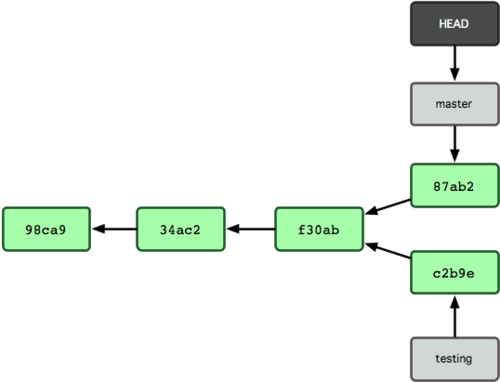
\includegraphics[height=55mm]{graphics/branching5}}
    \end{center}
\end{frame}

\begin{frame}{Commits: they form a DAG, and are stored on the ``heap''}

    Commits form a Directed Acyclic Graph (DAG). There are no loops in the
    graph, and every commit points to its parent(s).

    Every single commit is stored in the \texttt{.git} directory of your
    repository\footnote[frame]{Technically another lie.} which can be thought of
    like a ``heap'' for commits. The parents of a commit are also stored in this
    ``heap''.

    We will return to this fact when we talk about \textit{branches}.

\end{frame}

\begin{frame}{Commits: creating}
    You can create a commit by running \texttt{git commit}. This will create a
    commit based on the checked-out commit with the changes that you have
    ``staged''.
    \pause

    \begin{itemize}[<+->]
        \item You can stage changes by running \texttt{git add} and passing a
            list of files.
        \item You can stage all changes by running \texttt{git add -A}.
        \item \textbf{Pro tip}: If you want to add specific parts of files, use
            \texttt{git add -p}.
    \end{itemize}

    \pause[\thebeamerpauses]
    If you want to remove from the stage, you can run \texttt{git reset}
    (optionally passing a list of files to unstage).
\end{frame}

\begin{frame}[fragile]{Commits: what will be committed?}
    If you ever want to know what will be included in your commit, you can run
    \texttt{git status} to show the list of files staged for commit.
    \pause

    {
        \scriptsize
        \begin{minted}{text}
        > git status
        On branch master
        Your branch is ahead of 'origin/master' by 1 commit.
          (use "git push" to publish your local commits)

        Changes to be committed:
          (use "git restore --staged <file>..." to unstage)
                modified:   git.tex

        Changes not staged for commit:
          (use "git add <file>..." to update what will be committed)
          (use "git restore <file>..." to discard changes in working directory)
                modified:   git.pdf
                modified:   git.tex
        \end{minted}
    }

    \pause
    The \texttt{git.tex} file has only some lines staged for commit.
\end{frame}

\begin{frame}[fragile]{Commits: what will be committed, but with more detail?}
    To see the details of the changes that are staged (that is, will be
    committed), you can run \texttt{git diff --cached}.

    If you want to see the details of the changes that are \textit{not} staged,
    you can run \texttt{git diff}.

    \texttt{git diff} optionally accepts a list of files to diff.
    \pause

    {
        \tiny
        \begin{minted}{text}
            diff --git a/git.tex b/git.tex
            index 2c01a7b..91148d1 100644
            --- a/git.tex
            +++ b/git.tex
            @@ -33,9 +33,7 @@

             \section{Why use Git?}

            -\begin{frame}{Why use Git? I}
            -
            -    Example Scenario:
            +\begin{frame}{Example Scenario 1}

                 \begin{enumerate}[<+->]
                     \item You start a project called ``my-proj'' and write a ton of code.
        \end{minted}
    }
\end{frame}

\begin{frame}[fragile]{Commits: showing existing commits}
    You can view a commit using \texttt{git show <commit hash>}.

    {
        \tiny
        \begin{minted}{text}
            commit cb1b9610e4d34aa66b52e7fb722654679b4529e2
            Author: Sumner Evans <me@sumnerevans.com>
            Date:   Tue Jan 31 10:42:58 2023 -0700

                matrix-synapse: 1.76.0rc2 -> 1.76.0

                Signed-off-by: Sumner Evans <me@sumnerevans.com>

            diff --git a/modules/services/matrix/synapse/default.nix b/modules/services/matrix/synapse/default.nix
            index b142cf0..675ab77 100644
            --- a/modules/services/matrix/synapse/default.nix
            +++ b/modules/services/matrix/synapse/default.nix
            @@ -7,20 +7,20 @@ let
               # Custom package that tracks with the latest release of Synapse.
               package = pkgs.matrix-synapse.overridePythonAttrs (old: rec {
                 pname = "matrix-synapse";
            -    version = "1.76.0rc2";
            +    version = "1.76.0";
                 format = "pyproject";

                 src = pkgs.fetchFromGitHub {
                   owner = "matrix-org";
                   repo = "synapse";

            ...
        \end{minted}
    }
\end{frame}

\begin{frame}{Commits: summary}
    Use \texttt{git add} and \texttt{git reset} (or variants) to stage/unstage
    changes for your.
    \pause

    Use \texttt{git commit} to create a commit from the currently staged changes
    (which you can see by running \texttt{git diff --cached}).
\end{frame}

\section{Branches}

\begin{frame}{Branches: what are they?\footnote[frame]{Info in the rest of the
    \textit{Branches} section is mainly from
    \url{https://git-scm.com/book/en/v2/Git-Branching-Branches-in-a-Nutshell}}}

    Remember how we said that the \texttt{.git} directory is like a ``heap'' for
    commits?

    \textbf{Branches are pointers to a specific commit in that heap.} You can
    then follow that commit's parent pointers to reconstruct the graph.
\end{frame}

\begin{frame}{Branches: pointers}


    \begin{center}
        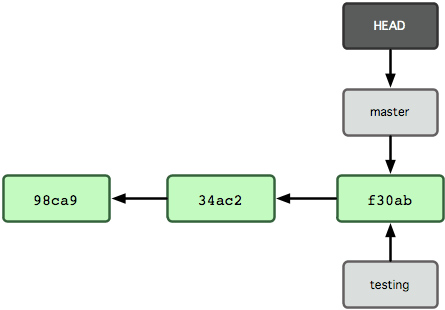
\includegraphics[height=50mm]{graphics/branching1}
    \end{center}
\end{frame}

\begin{frame}{Branches: creating them}
    Branches can be created using the \texttt{git branch <branch name>} command.
    \textbf{This will not change your \texttt{HEAD} pointer.}

    \begin{center}
        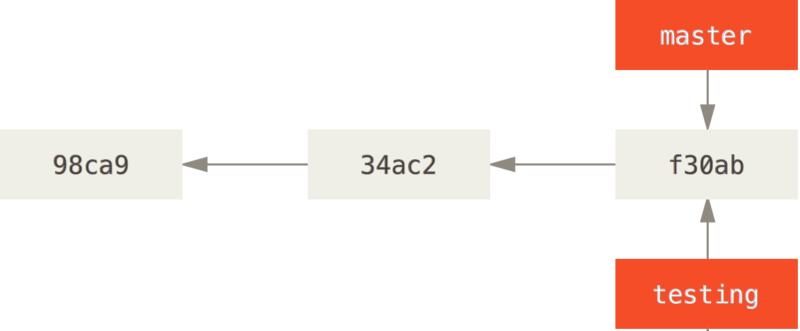
\includegraphics[height=35mm]{graphics/branching-creating}
    \end{center}

    If you want to create a branch and also change the \texttt{HEAD} pointer to
    the newly created branch, you can use:\\
    \texttt{git checkout -b <branch name>}.
    \pause

    You can use \texttt{git branch [-a]} to list (all) branches.
\end{frame}

\begin{frame}{Branches: moving \texttt{HEAD} around}
    \texttt{HEAD} is a special pointer to the current repository state.
    Checking out a commit/branch will update the files in your working
    directory.

    You can move the \texttt{HEAD} pointer to a different commit using\\
    \texttt{git checkout <commit hash or branch name>}.

    \only<1>{\begin{center}
        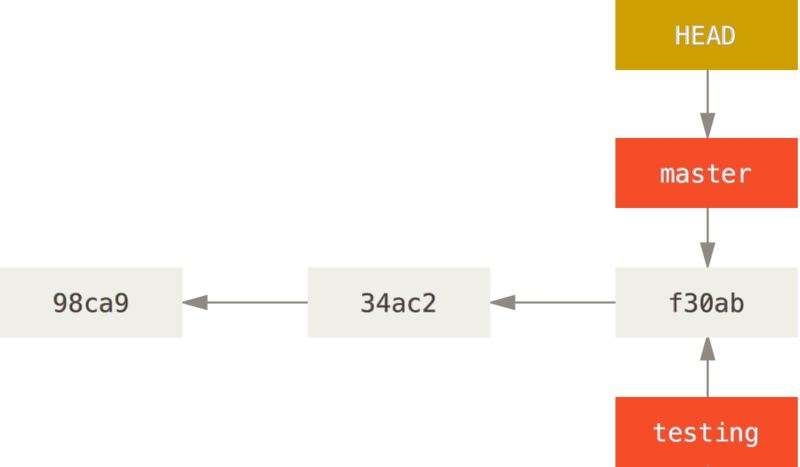
\includegraphics[height=45mm]{graphics/branching-moving-1}
    \end{center}}
    \only<2>{\begin{center}
        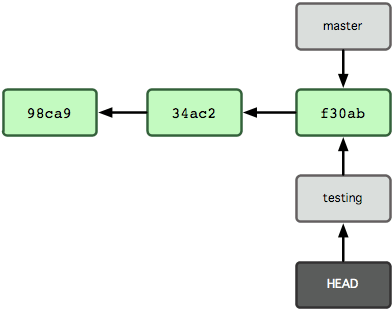
\includegraphics[height=45mm]{graphics/branching2}
    \end{center}}
\end{frame}

\begin{frame}{Branches: moving other branches around}
    If you want to move the branch that \texttt{HEAD} is pointing to to a
    different location, you can use \texttt{git reset}.
    \pause

    \texttt{git reset --hard <commit hash>} will move the branch that \texttt{HEAD}
    is pointing to to the specified commit, \textbf{discarding all changes in
    your working directory}.
    \pause

    \texttt{git reset --soft <commit hash>} will move the branch that
    \texttt{HEAD} is pointing to to the specified commit, \textbf{leaving all
    changes since the specified commit in your working directory}.
\end{frame}

\begin{frame}{Branches: \texttt{checkout} gotchas and pro-tips}
    \begin{itemize}
        \item If you checkout a commit hash, you will be in a \texttt{detached
            HEAD} state because your \texttt{HEAD} pointer is not pointing to a
            branch.
            \pause

        \item If you have uncommitted changes, switching branches \textit{might}
            fail.
            \pause

            You can use \texttt{git stash} to save the changes in your working
            directory, then \texttt{checkout} the other branch, and then
            \texttt{git stash pop} to restore the changes.

            Alternatively, you can just create a WIP commit and then switch to
            the other branch.
    \end{itemize}
    \pause

    \textbf{Pro tip}: You can use \texttt{-} to refer to the previously checked
    out object.
\end{frame}

\begin{frame}{Branches: making commits}
    If you commit something while \texttt{HEAD} is pointed to a branch, both
    \texttt{HEAD} and your branch will move to the new commit.

    \only<1>{\begin{center}
        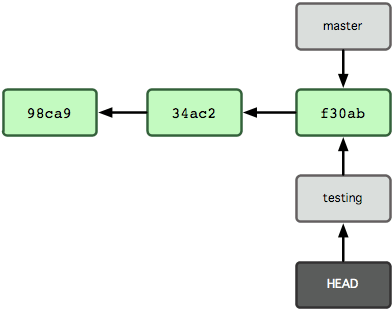
\includegraphics[height=45mm]{graphics/branching2}
    \end{center}}
    \only<2>{\begin{center}
        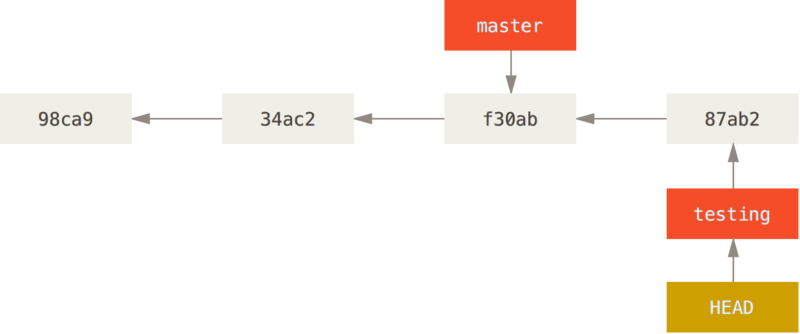
\includegraphics[height=45mm]{graphics/branching3}
    \end{center}}
\end{frame}

\begin{frame}{Branches: using multiple branches}
    Of course, you can always switch back to \texttt{master} using \texttt{git
    checkout master}.

    \begin{center}
        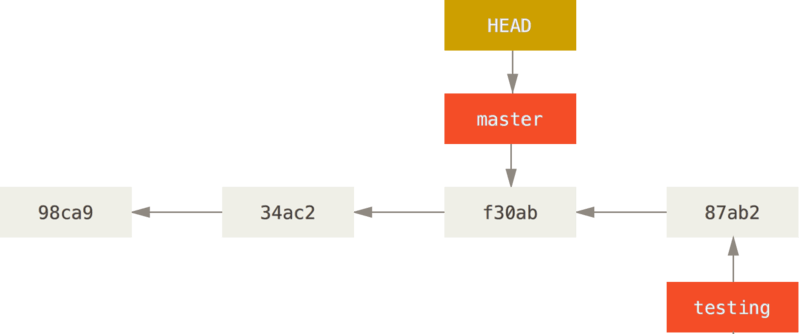
\includegraphics[width=110mm]{graphics/branching4}
    \end{center}
\end{frame}

\begin{frame}{Branches: divergence}
    If you make a commit on the master branch, the \texttt{master} pointer moves
    to that new commit creating \textbf{divergent} branch histories.

    \begin{center}
        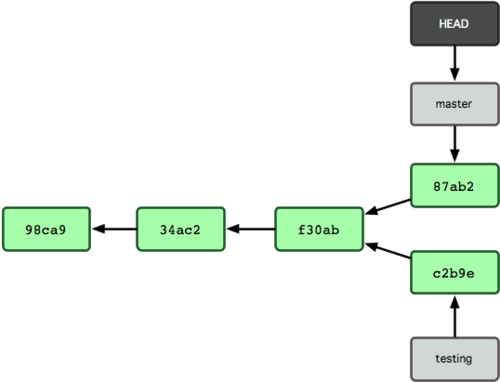
\includegraphics[width=110mm]{graphics/branching5}
    \end{center}
\end{frame}

\begin{frame}[fragile]{Branches: where am I?}
    Often, you want to get a summary of where you are in the repository. That's
    where \texttt{git log} comes in.

    {
        \tiny
        \begin{minted}{text}
            > git log
            commit b08107c144003ba42495995d59234595d2d875b4 (HEAD -> master, origin/master, origin/HEAD)
            Author: Sumner Evans <me@sumnerevans.com>
            Date:   Mon Feb 13 14:35:57 2023 -0700

                fix some things

                Signed-off-by: Sumner Evans <me@sumnerevans.com>

            commit 6c1f8b53ac774dc6b0376810b4745951bd572519
            Merge: 47bc626 67f0f4d
            Author: Ethan Richards <42894274+ezrichards@users.noreply.github.com>
            Date:   Mon Feb 13 14:06:08 2023 -0700

                Merge branch 'master' of github.com:ColoradoSchoolOfMines/mineshspc.com

            ...
        \end{minted}
    }
    \pause
    This is mostly useless. Let's make it better.
\end{frame}

\begin{frame}[fragile]{\texttt{git log}: but actually good}
    For \texttt{git log} to be useful, you want it to show \textit{all}
    branches, show a graph, and get rid of most of the details.

    {
        \tiny
        \begin{minted}{text}
            > git log --all --graph --decorate --oneline
            * b08107c (HEAD -> master, origin/master, origin/HEAD) fix some things
            *   6c1f8b5 Merge branch 'master' of github.com:ColoradoSchoolOfMines/mineshspc.com
            |\
            | * 67f0f4d fix background color bug
            * | 47bc626 Fix accordion
            |/
            * 186b52a Archive overhaul
            * 385666b Fix accordion arrows
            * 3d0f64a Archive preliminary updates
            * aaae02b Update FAQ and archive pages
            *   b2a64f7 Merge branch 'master' of github.com:ColoradoSchoolOfMines/mineshspc.com
            |\
            | * 1450745 make footer reveal
            * | f7ddfa2 Fix alt text
            |/
            * 0f89721 created student confirm registration page
            * 7b15e86 editing teams: ensure that you can't change from in-person to remote or vice versa
            * e15bda6 save team below member list
            * 853dcd1 add ability to add team members
            \end{minted}
    }
\end{frame}

\begin{frame}{Branches: summary}
    \begin{itemize}
        \item Branches are \textbf{pointers} to commits.
        \item Use \texttt{git checkout} to move between branches.
        \item Use \texttt{git log} to see where you are.
    \end{itemize}
\end{frame}

\section{Merging}

\begin{frame}{Merging: resolving divergent histories\footnote[frame]{Info in the rest of the
    \textit{Merging} section is mainly from
    \url{https://git-scm.com/book/en/v2/Git-Branching-Basic-Branching-and-Merging}}}

    If you want to merge the changes from branch \texttt{A} into another branch
    \texttt{B}, you need to:

    \begin{enumerate}
        \item Switch to branch \texttt{B} (\texttt{git checkout B})
        \item Run \texttt{git merge A}.
    \end{enumerate}

    This will do one of two things: fast-forward or create a merge commit.
\end{frame}

\begin{frame}{Merging: fast-forwarding}

    If the branch you are merging is directly ahead of the branch you are
    merging into, Git will just move the pointer in a \textbf{fast-forward
    merge}.

    \begin{center}
        \only<1>{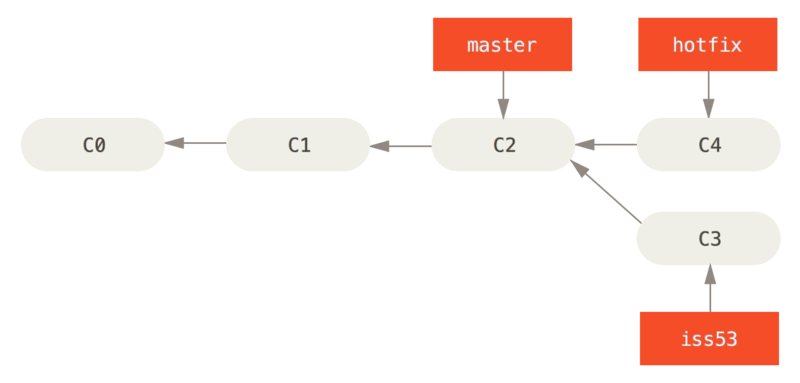
\includegraphics[width=90mm]{graphics/merging-1}}
        \only<2>{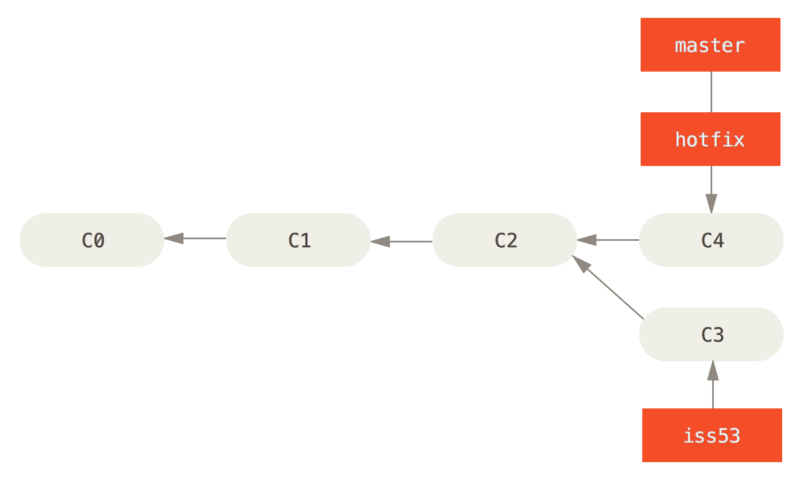
\includegraphics[width=90mm]{graphics/merging-2}}
    \end{center}
\end{frame}

\begin{frame}{Merging: creating a merge commit}
    If the branch you are merging has diverged from the one you are merging
    into, Git will create a merge commit through a \textbf{three-way merge}.

    \begin{center}
        \only<1>{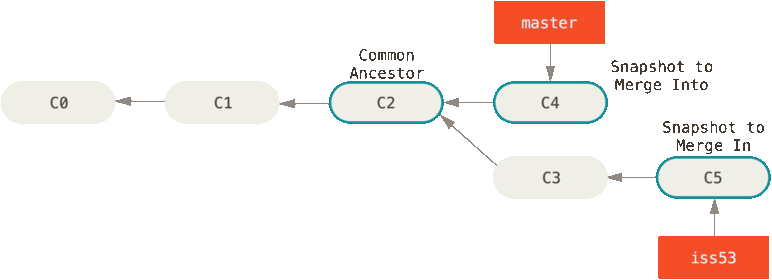
\includegraphics[height=30mm]{graphics/merging-3way-1}}
        \only<2>{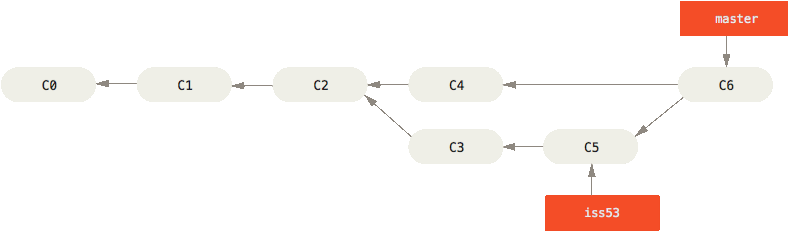
\includegraphics[height=30mm]{graphics/merging-3way-2}}
    \end{center}
\end{frame}

\begin{frame}[fragile]{Merging: resolving conflicts}
    Occasionally, this process doesn't go smoothly. If you changed the same part
    of the same file differently in the two branches you're merging, Git won't
    be able to merge them cleanly.

    {
        \tiny
        \begin{minted}{text}
            > git merge iss53
            Auto-merging index.html
            CONFLICT (content): Merge conflict in index.html
            Automatic merge failed; fix conflicts and then commit the result.
        \end{minted}
    }
    \pause
    You can always use \texttt{git status} to see what has been automatically
    merged and what files have conflicts.
    {
        \tiny
        \begin{minted}{text}
            > git status
            On branch master
            You have unmerged paths.
              (fix conflicts and run "git commit")

            Unmerged paths:
              (use "git add <file>..." to mark resolution)

                both modified:      index.html

            no changes added to commit (use "git add" and/or "git commit -a")
        \end{minted}
    }
\end{frame}

\begin{frame}[fragile]{Merging: editing files to resolve merge conflicts}
    You can use a merge tool to resolve conflicts, however I find that it's
    easier to just manually resolve the conflicts.

    Visual Studio Code has a good UI for this. The process you should follow is
    as follows:

    \begin{enumerate}
        \item Open a file with the conflict.
        \item Find one of the conflict-resolution markers.
        \item Make edits to resolve the conflict.
        \item Run \texttt{git add} on the file.
        \item Repeat steps 1-4 until all conflicts are resolved.
        \item Run \texttt{git commit} to commit the merge.
    \end{enumerate}

\end{frame}

\begin{frame}[fragile]{Merging: understanding conflict-resolution markers}
    In order to find the conflict-resolution markers, search for
    \texttt{<<<<<<<}. Each conflict-resolution block should look something like
    this:
    {
        \tiny
        \begin{minted}{text}
            <<<<<<< HEAD:index.html
            <div id="footer">contact : email.support@github.com</div>
            =======
            <div id="footer">
             please contact us at support@github.com
            </div>
            >>>>>>> iss53:index.html
        \end{minted}
    }

    The first part (between \texttt{<<<<<<<} and \texttt{=======}) is what the
    branch you are merging \textit{into} has. The second part (between
    \texttt{=======} and \texttt{>>>>>>>}) is what the branch you are merging
    \textit{from} has.
    \pause

    Sometimes, you just one one side of the conflict, other times you need to be
    more nuanced in your merge.
\end{frame}

\begin{frame}{Merging: summary}
    \begin{itemize}
        \item Merging allows you to pull changes from one branch into another
            branch.
        \item Use \texttt{git merge A} to merge branch \texttt{A} into the
            current branch.
        \item Git will do a fast-forward merge if possible, otherwise it will
            create a merge commit.
        \item You might have to resolve merge conflicts.
    \end{itemize}
\end{frame}

\section{Rebasing}

\begin{frame}[fragile]{Rebasing: maintaining linear histories}
    Most merge commits are useless. They clutter the history, and normally don't
    add anything of value to the understanding of how the codebase evolved.

    {
        \tiny
        \begin{minted}{text}
            * b08107c (HEAD -> master, origin/master, origin/HEAD) fix some things
            *   6c1f8b5 Merge branch 'master' of github.com:ColoradoSchoolOfMines/mineshspc.com
            |\
            | * 67f0f4d fix background color bug
            * | 47bc626 Fix accordion
            |/
            * 186b52a Archive overhaul
            * 385666b Fix accordion arrows
        \end{minted}
    }
    \pause

    Ideally the above history would be linear:

    {
        \tiny
        \begin{minted}{text}
            * b08107c (HEAD -> master, origin/master, origin/HEAD) fix some things
            * 47bc626 Fix accordion
            * 67f0f4d fix background color bug
            * 186b52a Archive overhaul
            * 385666b Fix accordion arrows
        \end{minted}
    }

\end{frame}

\begin{frame}{Rebasing: what it does}
    Rebasing allows you to take the commits from one branch and reapply them on
    top of another branch.

    \begin{center}
        \only<1>{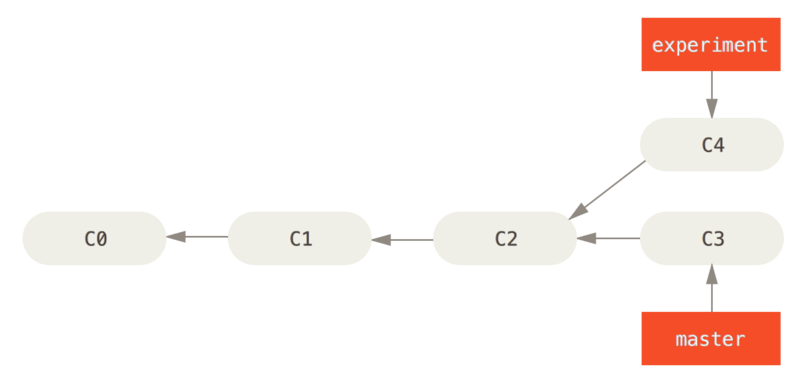
\includegraphics[height=40mm]{graphics/basic-rebase-1}}
        \only<2>{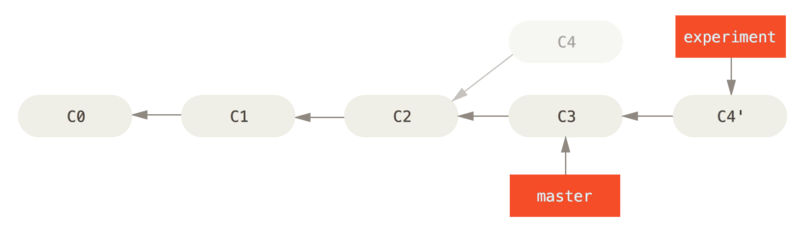
\includegraphics[height=30mm]{graphics/basic-rebase-3}}
        \only<3>{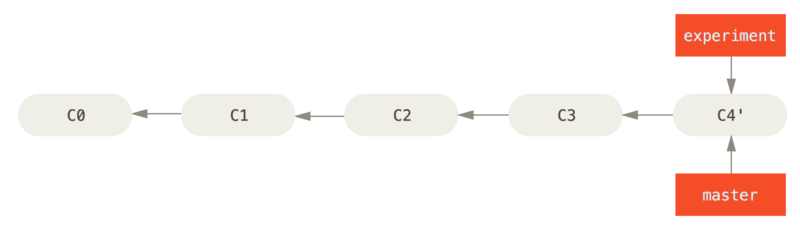
\includegraphics[height=30mm]{graphics/basic-rebase-4}}
    \end{center}
\end{frame}

\begin{frame}{Rebasing: how to rebase}
    To rebase, follow this procedure:

    \begin{enumerate}
        \item Checkout the branch that you want to rebase.
        \item Run \texttt{git rebase A}, where \texttt{A} is the branch or
            commit you want to rebase onto.
    \end{enumerate}
    \pause

    Note that \textbf{rebasing rewrites history}. Generally you should only
    rebase \textit{local} commits, or branches that you are the only one using.
\end{frame}

\begin{frame}[fragile]{Rebasing: interactive rebase}
    Say you are working on a feature branch and you've made the following
    commits:
    {
        \tiny
        \begin{minted}{text}
            * 1a2b3c4 (HEAD -> my-feature) add more buzz
            * 8a9b0c1 fix fizzing
            * 1d2e3f4 (master) fizz the buzz
        \end{minted}
    }
    \pause

    But you realize that your \texttt{fix fizzing} commit introduced a bug! So
    you fix the issue but you don't want to end up with a ``fix the fix''
    commit.\\
    \pause

    Interactive rebasing can help! Go ahead and create a new ``fix the fix''
    commit:
    {
        \tiny
        \begin{minted}{text}
            * a81abe1 (HEAD -> my-feature) fixup! fix fix fizzing
            * 1a2b3c4 add more buzz
            * 8a9b0c1 fix fizzing
            * 1d2e3f4 (master) fizz the buzz
        \end{minted}
    }
\end{frame}

\begin{frame}[fragile]{Rebasing: interactive rebase (continued)}
    Interactive rebasing can help! Go ahead and create a new ``fix the fix''
    commit:
    {
        \tiny
        \begin{minted}{text}
            * a81abe1 (HEAD -> my-feature) fixup! fix fizzing
            * 1a2b3c4 add more buzz
            * 8a9b0c1 fix fizzing
            * 1d2e3f4 (master) fizz the buzz
        \end{minted}
    }

    Now, run \texttt{git rebase -i master} to start an interactive rebase. This
    will open an editor with the following (as well as instructions):
    {
        \tiny
        \begin{minted}{text}
            pick 8a9b0c1 fix fizzing
            pick 1a2b3c4 add more buzz
            pick a81abe1 fixup! fix fizzing
        \end{minted}
    }
    \pause

    Now, you can move the commit order around by editing the file, and also
    \texttt{fixup} the commit, which will squash the two commits together into
    one!
    {
        \tiny
        \begin{minted}{text}
            pick 8a9b0c1 fix fizzing
            fixup a81abe1 fixup! fix fizzing
            pick 1a2b3c4 add more buzz
        \end{minted}
    }
\end{frame}

\begin{frame}[fragile]{Rebasing: interactive rebase result}
    Now, you can move the commit order around by editing the file, and also
    \texttt{fixup} the commit, which will squash the two commits together into
    one!
    {
        \tiny
        \begin{minted}{text}
            pick 8a9b0c1 fix fizzing
            fixup a81abe1 fixup! fix fizzing
            pick 1a2b3c4 add more buzz
        \end{minted}
    }
    \pause

    After saving and exiting the editor, Git will rewrite the history of your
    branch to look like this:
    {
        \tiny
        \begin{minted}{text}
            * a9bb207 (HEAD -> my-feature) add more buzz
            * 4e89d4f fix fizzing
            * 1d2e3f4 (master) fizz the buzz
        \end{minted}
    }
    and the \texttt{fix fizzing} commit will contain the changes from both
    commits!
    \pause

    \textbf{Note that you now have different commit hashes!} The old commits are
    still in tact (you can \texttt{checkout} them), but you have moved your
    branch (pointer) to the new commit.
\end{frame}

\begin{frame}[fragile]{Rebasing: interactive rebase shortcut}
    The workflow I described in the previous slides is so common that there are
    tools built-in to Git to help you accomplish them.

    \begin{itemize}
        \item \texttt{git commit --fixup <commit>} automatically marks your
            commit as a fix of a previous commit. (It uses that \texttt{fixup!}
            syntax from the previous slide.)

        \item \texttt{git rebase -i --autosquash} opens the editor and
            automatically reorders the fixup commits when the interactive rebase
            editor opens and sets them to \texttt{fixup} instead of
            \texttt{pick}.
    \end{itemize}

    See
    \url{https://fle.github.io/git-tip-keep-your-branch-clean-with-fixup-and-autosquash.html}
    for more details.
\end{frame}

\begin{frame}{Rebasing: bailing out}
    If you ever need to cancel a rebase, use \texttt{git rebase --abort}.

    This will restore your repository state to what it was before you started
    the rebase process.
\end{frame}

\begin{frame}{Rebasing: other applications}
    There are lots of other reasons to rebase.
    \begin{itemize}
        \item You want to pull in changes from another branch without merging.
        \item You want to modify a commit that added a file by accident.
        \item You want to reorder your commits to make it more clear to a code
            reviewer what you changed.
        \item Somebody else pushed a commit to the \textit{remote} branch, and
            you want to add your commit on top of theirs.
    \end{itemize}
\end{frame}

\section{Remotes}

\begin{frame}{Remotes: what are they?\footnote[frame]{Much of the content of
    this section is from
    https://git-scm.com/book/en/v2/Git-Basics-Working-with-Remotes}}

    Remote repositories are versions of your project that are hosted on the
    Internet or network somewhere. You can have several of them, each of which
    generally is either read-only or read/write for you.
    \pause

    GitHub is a popular choice for where to host your remote repositories, but
    other options exist such as GitLab, sourcehut, Bitbucket, and many other
    self-hosted options.
\end{frame}

\begin{frame}[fragile]{Remotes: managing them}
    \begin{itemize}
        \item View all of your remotes with:

            {
                \footnotesize
                \begin{minted}{text}
                    > git remote -v
                    origin  git@github.com:sumnerevans/acm-git-good.git (fetch)
                    origin  git@github.com:sumnerevans/acm-git-good.git (push)
                \end{minted}
            }
            \pause

        \item You can add remotes using:

            {
                \footnotesize
                \begin{minted}{text}
                    > git remote add other git@github.com:other/repo.git
                \end{minted}
            }
            \pause

        \item You can change the URL of a remote:

            {
                \footnotesize
                \begin{minted}{text}
                    > git remote set-url origin git@github.com:other/repo.git
                \end{minted}
            }
            \pause

        \item When you clone a repository, it automatically creates a remote
            called \texttt{origin} that points to your remote repository.
            \pause

        \item \textbf{Note}: \texttt{origin} is not special, it's just a
            default.
    \end{itemize}
\end{frame}

\begin{frame}{Remote Branches: what are they?}
    The remote repository is \textbf{entirely separate from your local
    repository}. The remote repository has its own set of branches, commits,
    etc.

    \begin{center}
        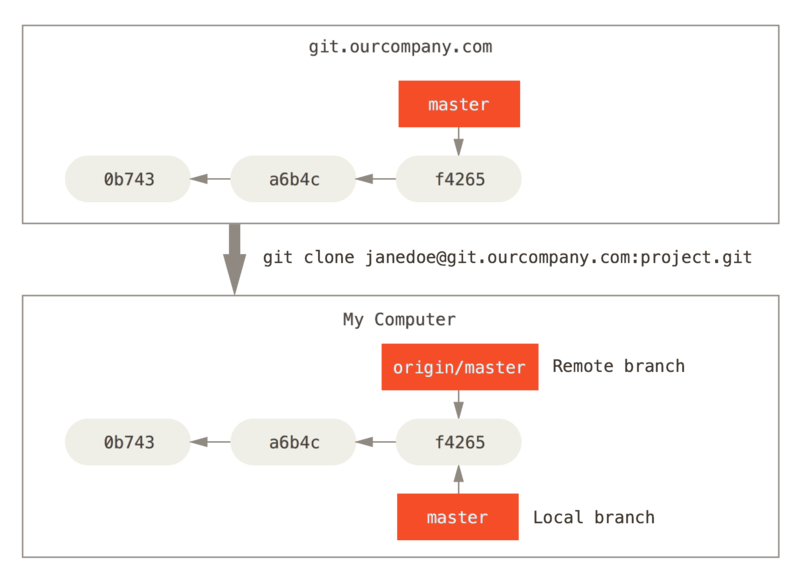
\includegraphics[height=60mm]{graphics/remote-branches-1}
    \end{center}
\end{frame}

\begin{frame}{Remote Branches: three new concepts}
    \begin{enumerate}
        \item \textbf{Fetch}: to download the current state of the remote
            repository, use the \texttt{git fetch} command.

            \textbf{Git does not automatically fetch the state of the remote
            repository!}
            \pause

        \item \textbf{Push}: to update the remote repository with your local
            state, use the \texttt{git push} command.
            \pause

        \item \textbf{Tracking branches}: tracking branches are local branches
            that have a direct relationship to a remote branch.
    \end{enumerate}
\end{frame}

\begin{frame}{Remote Branches: divergence}
    The state of the local and remote repositories can diverge.
    \visible<3>{Use \texttt{git fetch} to get the latest state of the remote
    repository.}

    \begin{center}
        \only<1>{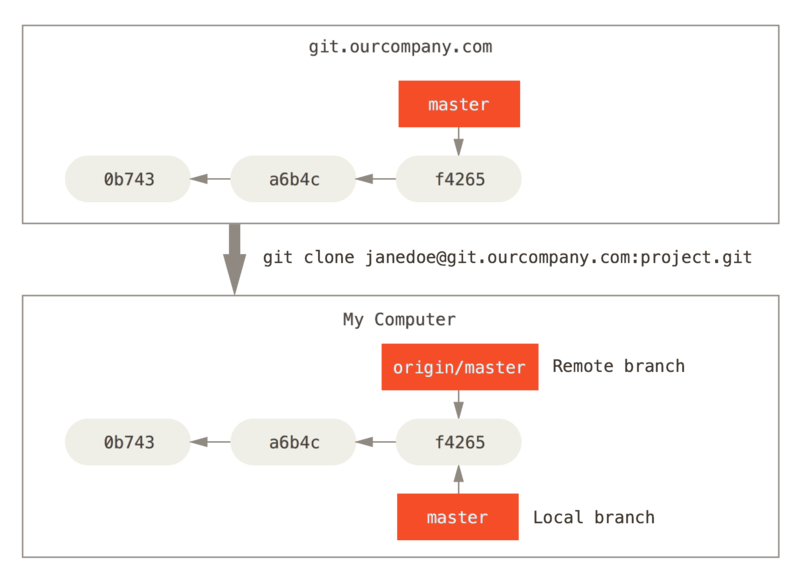
\includegraphics[height=55mm]{graphics/remote-branches-1}}
        \only<2>{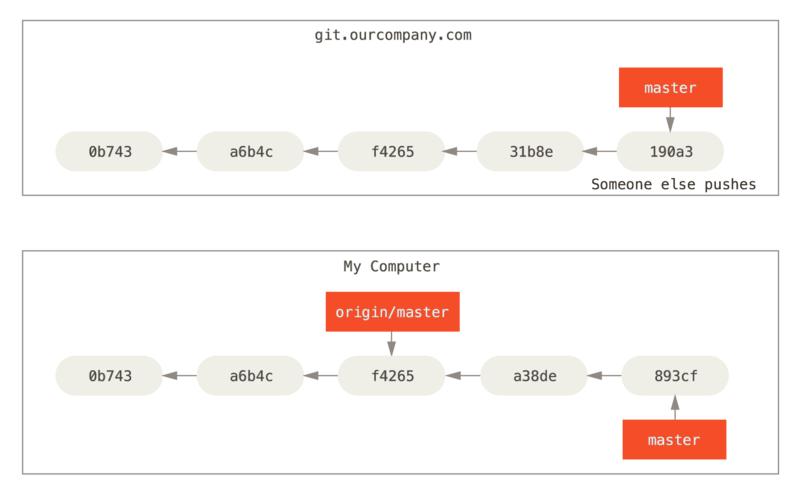
\includegraphics[height=55mm]{graphics/remote-branches-2}}
        \only<3>{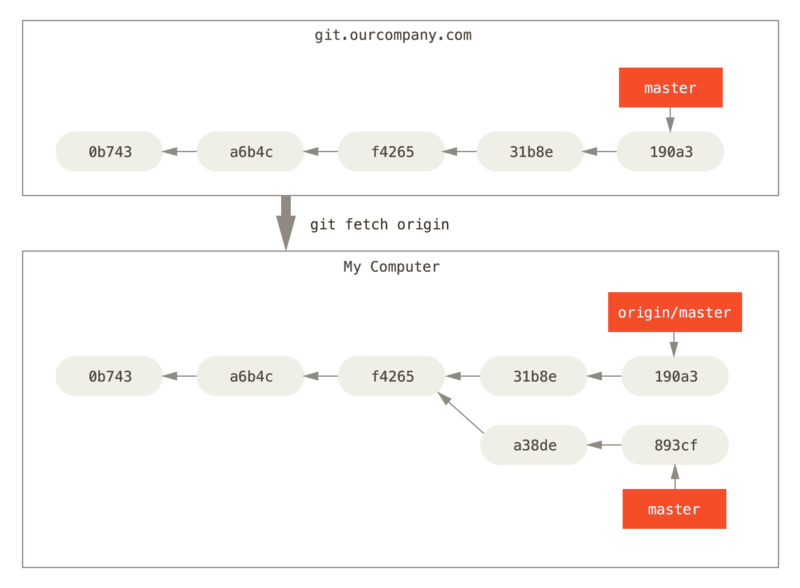
\includegraphics[height=55mm]{graphics/remote-branches-3}}
    \end{center}
    \visible<3>{Now use the tools we already know for divergent branches.}
\end{frame}

\begin{frame}[fragile]{Remote Branches: divergence (continued)}
    Git provides a command to fetch and then merge the remote branch into the
    local branch called \texttt{git pull}.
    \pause

    \textbf{Warning}: by default, \texttt{git pull} will create a merge commit
    if the remote branch has diverged from the local one!

    Merge commits are ugly! Use \texttt{git pull --rebase} to tell \texttt{git
    pull} to rebase your local changes on the remote changes instead.
    \pause

    \begin{block}{Tell Git to never merge when pulling}
        You can configure Git to fail instead of making a merge commit by
        setting the \texttt{pull.ff} configuration option to \texttt{only}.
        {
            \begin{minted}{text}
                > git config --global pull.ff only
            \end{minted}
        }
    \end{block}
\end{frame}

\begin{frame}[fragile]{Remote Branches: pushing}
    Pushing can be thought of merging your local tracking into the remote
    tracking branch.

    If your branch is already configured to track a remote branch, you can just
    use \texttt{git push}.
    \pause

    If you have a new branch that doesn't have a corresponding remote tracking
    branch, use
    {
        \begin{minted}{text}
            > git push -u origin <branch name>
        \end{minted}
    }
\end{frame}

\begin{frame}[fragile]{Remote Branches: pushing harder}
    In certain circumstances, you want to push a divergent branch to the remote.
    Examples include:

    \begin{itemize}
        \item You did an interactive rebase and need to push the newly rebased
            changes.
        \item You reset your branch to a previous commit and want it to be the
            latest commit on the branch.
    \end{itemize}
    \pause

    In these cases, you can use the \texttt{--force} or
    \texttt{--force-with-lease} options to tell Git to push your local state to
    the remote regardless of what is currently there.

    \texttt{--force-with-lease} is less dangerous than \texttt{--force} because
    it will check that your current view of the remote state is up-to-date.
\end{frame}

\section{Advanced Tips}

\begin{frame}{Undoing Things}
    Commits are kept around in the \texttt{.git} directory (remember, it's like
    a heap), which means that even if you loose a pointer to a commit (for
    example by moving all branch pointers away from it), it still exists!

    You can use \texttt{git reflog} to see the history of when the tips of
    branches and other references were updated in the local repository.
    \pause

    If you screwed something up and you don't know what to do,
    \url{https://ohshitgit.com/} is a great resource.
\end{frame}

\begin{frame}{Cherry-picking}

    You can apply arbitrary commits to your current branch by cherry-picking
    them.

    This is similar to rebasing.

\end{frame}

\begin{frame}[fragile]{Aliases}

    Git supports the concept of \textit{aliasing} one command to another name.

    For example, you can alias the pretty log command I showed earlier to
    \texttt{git l} by using the following command:
    {
        \scriptsize
        \begin{minted}{text}
            > git config --global alias.l "log --oneline --graph --all --decorate"
        \end{minted}
    }

    Now you can just type \texttt{git l} to get the pretty version of the log
    output.
\end{frame}

\begin{frame}{Ignoring Files}
    You can tell Git to not ever commit certain files by ignoring them using the \texttt{.gitignore} file.

    Any file that matches one of the patterns in \texttt{.gitignore} will not be
    tracked by Git.
    \pause

    \textbf{Warning}: if you have already committed the file, it will still be
    tracked.

    If you want to delete a file from Git, but keep it on your computer, use
    \texttt{git rm --cached <file>}.
\end{frame}

\begin{frame}{Blaming}

    Want to see the last commit that modified each line of a file? Use
    \texttt{git blame}.

    This is often a helpful way to see which commit cause a bug or see what
    needs to be changed when making a similar change.

\end{frame}

\begin{frame}{Resources/Tips}

    I obviously was unable to tell you about everything you can do with Git.
    There are hundreds of options on every single command.

    \begin{itemize}
        \item \texttt{man git *}: The man pages on Git are good. Use them as your first line of
            defense.
        \item \href{https://git-scm.com/book/en/v2}{git-scm.com/book/en/v2}: A
            huge resource about how to do everything Git.
        \item \href{https://gitignore.io}{gitignore.io}: Generates a
            \texttt{.gitignore} file for a given project type, OS, and IDE.
        \item \href{https://github.com/dandavison/delta}{delta}: provides a much
            prettier \texttt{diff} interface.
    \end{itemize}
\end{frame}

\end{document}
